\documentclass[a4paper,11pt]{article}

\renewcommand\thesection{\arabic{section}.}

\usepackage{tocloft}
\cftsetindents{section}{0em}{2em}
\cftsetindents{subsection}{0em}{2em}
\renewcommand\cfttoctitlefont{\hfill\Large\bfseries}
\renewcommand\cftaftertoctitle{\hfill\mbox{}}
\setcounter{tocdepth}{10}

\usepackage{listings}
\usepackage{xcolor}

\usepackage{fullpage}

\usepackage{float}

\usepackage{amsfonts}

\usepackage{sectsty}
\sectionfont{\fontsize{14}{15}\selectfont}

\usepackage{graphicx}
\usepackage[margin=0.6in,includefoot,headsep=0.1in]{geometry}
\usepackage{fancyhdr}
\pagestyle{fancy}
\fancyhf{}
\cfoot{\thepage}
\rfoot{P. T. O.}
\lfoot{ROHIT DAS 30000114022}

\usepackage{booktabs}
\usepackage{tabularx}

%\usepackage{array}
%\newcolumntype{P}[1]{>{\centering\arraybackslash}p{#1}}

\lstset { %
    language=C,
    backgroundcolor=\color{black!5}, % set backgroundcolor
    basicstyle=\large,% basic font setting
}

\newcommand*{\plogo}{\fbox{$\mathcal{PL}$}} % Generic publisher logo

%----------------------------------------------------------------------------------------
%	TITLE PAGE
%----------------------------------------------------------------------------------------

\newcommand*{\titleGM}{\begingroup % Create the command for including the title page in the document
\hbox{ % Horizontal box
\hspace*{0.18\textwidth} % Whitespace to the left of the title page
\rule{1pt}{\textheight} % Vertical line
\rule{1pt}{\textheight}
\hspace*{0.05\textwidth} % Whitespace between the vertical line and title page text
\parbox[b]{0.75\textwidth}{ % Paragraph box which restricts text to less than the width of the page

{\noindent\Huge\bfseries Software Engineering}\\[2\baselineskip] % Title
{\large \textit{-supervised by:}\\\\\Large \textsc Dr. Suparna Biswas (Saha)}\\[4\baselineskip] % Tagline or further description

{\huge \textsc{Rohit Das}} % Author name
{\\\\\Large{B. Tech(Computer Sc. and Engg)}\\\\\Large{Roll: 30000114022\\\\\Large{Regn. No.:143000110023}\\\\\Large{6th Semester,2016}}}
\vspace{120pt} % Whitespace between the title block and the publisher
\begin{figure}[H]
\hspace*{100pt}
\includegraphics[width=90pt,height=\textheight,keepaspectratio]{/home/mouri/Pictures/makaut.jpg}
\end{figure}
{\noindent \textit{\large{Maulana Abul Kalam Azad University of Technology,\\\\West Bengal.\\\\}}{\large \LaTeX} \hspace{5pt}2017}\\[\baselineskip] % Publisher and logo
}}
\endgroup}

\begin{document}
%\pagestyle{empty} % Removes page numbers
\thispagestyle{empty}
\titleGM % This command includes the title page

\iffalse
\title{\textbf{\Huge Maulana Abul Kalam Azad University of\\[10pt] Technology}}
\date{\vspace{-5ex}}
\maketitle
\begin{center}
\textbf{\LARGE{(SOftware Engineering Assignment)}}
\end{center}
\begin{figure}[H]
\centering
\includegraphics[width=350pt,height=\textheight,keepaspectratio]{/home/mouri/Pictures/makaut.jpg}
\end{figure}
.

\begin{flushright}
\underline{\textbf{\author{\Huge Rohit Das}}}\\
\textbf{\LARGE{
B. Tech(CSE),5th Year\\
Roll No.: 3000114022\\
Regn. No.: 143000110023\\
Taught by: Dr .Suparna Biswas (Saha)\\
}}
\end{flushright}
%\tableofcontents
%\begin{table}[htbp]
%\centering
\fi

\tableofcontents
\break

\section{Assignment-1: C programming (Date: 27/10/2017)}
\subsection{Write a program to implement Calendar program to display Day of the month. Program will accept year, month and date from user and will display the day of the month.}
\underline{Program:}
\lstinputlisting[showstringspaces=false]{../assign1/1.c}
Output:
\begin{figure}[H]
\centering
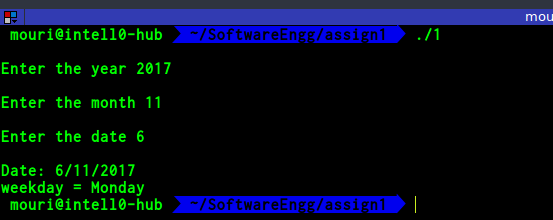
\includegraphics[width=350pt,height=\textheight,keepaspectratio]{./pics/1.png}
\end{figure}

\bigskip

%\section{Date: 21/4/2017}
\subsection{Write a program to find inverse of 3x3 matrix.}
\underline{Program:}
\lstinputlisting[showstringspaces=false]{../assign1/2.c}
Output:
\begin{figure}[H]
\centering
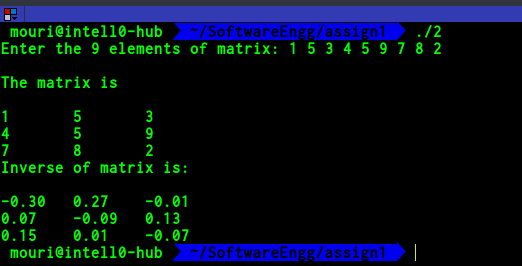
\includegraphics[width=350pt,height=\textheight,keepaspectratio]{./pics/2.png}
\end{figure}

\bigskip

%\section{Date: 28/4/2017}
\subsection{Write a program to check whether matrix is Magic Square or not.}
\underline{Program:}
\lstinputlisting[showstringspaces=false]{../assign1/3.c}
Output:
\begin{figure}[H]
\centering
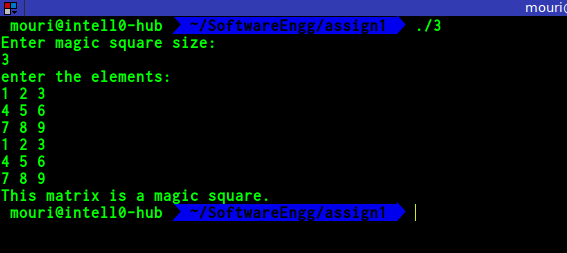
\includegraphics[width=350pt,height=\textheight,keepaspectratio]{./pics/3.png}
\end{figure}
\bigskip

\subsection{Write a program to read last n characters from a file(input should be a.txt).}
\underline{Program:}
\lstinputlisting[showstringspaces=false]{../assign1/a.txt}

\lstinputlisting[showstringspaces=false]{../assign1/4.c}
Output:
\begin{figure}[H]
\centering
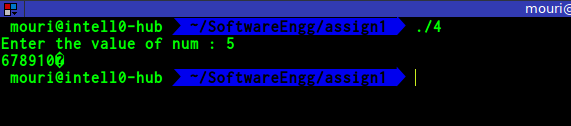
\includegraphics[width=350pt,height=\textheight,keepaspectratio]{./pics/4.png}
\end{figure}
\bigskip

%\section{Date: 5/5/2017}
\subsection{Write a program to print binary numbers in pyramid pattern.}
\underline{Program:}
\lstinputlisting[showstringspaces=false]{../assign1/5.c}
Output:
\begin{figure}[H]
\centering
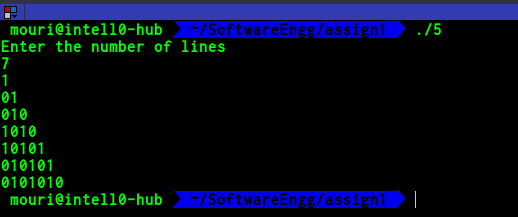
\includegraphics[width=350pt,height=\textheight,keepaspectratio]{./pics/5.png}
\end{figure}
\bigskip

%\section{Date: 12/5/2017}
\subsection{Write a program to input password for validation of username.\\
Enter password: ******\\
Password entered: sourav}
\underline{Program:}
\lstinputlisting[showstringspaces=false]{../assign1/6.c}
Output:
\begin{figure}[H]
\centering
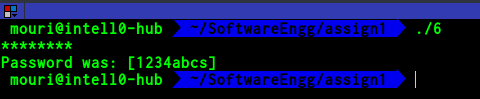
\includegraphics[width=350pt,height=\textheight,keepaspectratio]{./pics/6.png}
\end{figure}
\bigskip

%\section{19/5/2017}
\subsection{Write a program to create your own header file in C.}
\underline{Program:}
\lstinputlisting[showstringspaces=false]{../assign1/test.h}

\lstinputlisting[showstringspaces=false]{../assign1/7.c}
Output:
\begin{figure}[H]
\centering
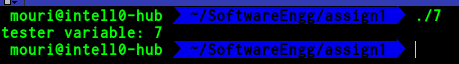
\includegraphics[width=350pt,height=\textheight,keepaspectratio]{./pics/7.png}
\end{figure}
\bigskip


\subsection{Write a program to compare two strings without using library function(strcmp).}
\underline{Program:}
\lstinputlisting[showstringspaces=false]{../assign1/8.c}
Output:
\begin{figure}[H]
\centering
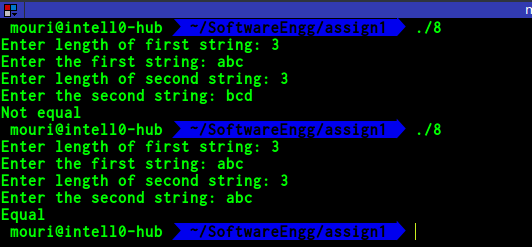
\includegraphics[width=350pt,height=\textheight,keepaspectratio]{./pics/8.png}
\end{figure}
\bigskip

\subsection{Write a program to print a rectangle using line and special symbols.}
\underline{Program:}
\lstinputlisting[showstringspaces=false]{../assign1/9.c}
Output:
\begin{figure}[H]
\centering
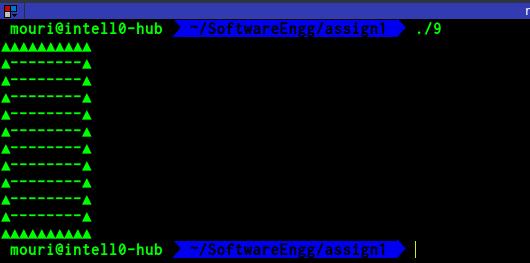
\includegraphics[width=350pt,height=\textheight,keepaspectratio]{./pics/9.png}
\end{figure}
\bigskip

\subsection{Write a program to find addition of lower triangular matrix.}
\underline{Program:}
\lstinputlisting[showstringspaces=false]{../assign1/10.c}
Output:
\begin{figure}[H]
\centering
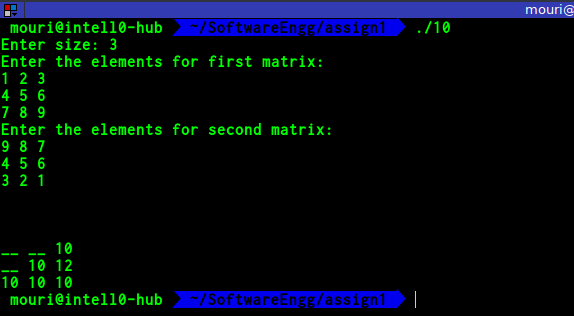
\includegraphics[width=350pt,height=\textheight,keepaspectratio]{./pics/10.png}
\end{figure}
\bigskip

\end{document}